%
\clearpage\onecolumn
\begingroup
\newcolumntype{B}{S[table-auto-round = true,exponent-product=\cdot,scientific-notation=true,table-figures-decimal=2,table-figures-integer=2,table-figures-exponent=1]}
\newcolumntype{T}{S[table-auto-round = true,table-format=2.2]}
% % \rotFPtop=0pt plus 1fil
% \rotFPtop=0pt
% \rotFPbot=0pt plus 1fil
\begin{sidewaystable}
\centering
% \begin{table}
\caption{Raw numbers for the comparison benchmarks. \emph{ops} is number of
  operations (higher is better), \emph{time (s)} is time in seconds (lower is
  better), \emph{ops / s} is number of operations per second (higher is better).}
% \begin{sideways}
\smaller\smaller\smaller
\sisetup{table-number-alignment = center}
% \hspace*{-1cm}
\begin{tabular}{%
c@{}r
B@{}T@{}B
B@{}T@{}B
B@{}T@{}B
B@{}T@{}B
B@{}T@{}B
B@{}T@{}B
B@{}T@{}B
}
\toprule
	&&\multicolumn{3}{c}{ContextL}&\multicolumn{3}{c}{ContextJS Edge}&\multicolumn{3}{c}{ContextJS Chrome OSX}&\multicolumn{3}{c}{ContextJS Chrome Win}&\multicolumn{3}{c}{ContextPy Python OSX}&\multicolumn{3}{c}{ContextPy PyPy OSX}&\multicolumn{3}{c}{ContextPyPy PyPy OSX} \\ 
\midrule
	&&{ops }&{ time (s) }&{ ops / s }&{ ops }&{ time (s) }&{ ops / s }&{ ops }&{ time (s) }&{ ops / s }&{ ops }&{ time (s) }&{ ops / s }&{ ops }&{ time (s) }&{ ops / s }&{ ops }&{ time (s) }&{ ops / s }&{ ops }&{ time (s) }& {ops / s} \\ 
\midrule
\parbox[t]{2mm}{\multirow{10}{*}{\rotatebox[origin=c]{90}{NoLayer}}}
 & 1 & 819200000 & 6.963 & 117650438 & 838860800 & 7.719 & 108674802 & 3355443200 & 9.555 & 351171450 & 3355443200 & 9.819 & 341729626 & 25600000 & 5.364 & 4772558 & 819200000 & 8.577 & 95511251 & 819200000 & 8.818 & 92900885\\
 & 2 & 409600000 & 5.213 & 78572799 & 838860800 & 8.256 & 101606202 & 3355443200 & 9.603 & 349416141 & 1677721600 & 5.108 & 328449804 & 25600000 & 9.077 & 2820315 & 819200000 & 9.765 & 83891449 & 819200000 & 9.842 & 83235115\\
 & 3 & 409600000 & 6.410 & 63900156 & 838860800 & 8.896 & 94296403 & 3355443200 & 9.590 & 349889802 & 1677721600 & 5.335 & 314474527 & 12800000 & 6.010 & 2129784 & 409600000 & 5.279 & 77590453 & 409600000 & 5.100 & 80313725\\
 & 4 & 409600000 & 8.351 & 49048018 & 419430400 & 5.796 & 72365493 & 3355443200 & 9.576 & 350401337 & 1677721600 & 5.190 & 323260424 & 12800000 & 7.559 & 1693346 & 409600000 & 6.273 & 65295712 & 409600000 & 6.292 & 65098538\\
 & 5 & 409600000 & 9.983 & 41029751 & 419430400 & 5.327 & 78736700 & 3355443200 & 9.620 & 348798669 & 1677721600 & 5.859 & 286349479 & 12800000 & 8.953 & 1429688 & 409600000 & 6.620 & 61873112 & 409600000 & 6.550 & 62534351\\
 & 6 & 204800000 & 5.975 & 34276151 & 419430400 & 9.751 & 43014091 & 1677721600 & 5.238 & 320298129 & 1677721600 & 6.689 & 250818000 & 6400000 & 5.332 & 1200300 & 409600000 & 7.734 & 52960952 & 409600000 & 8.157 & 50214540\\
 & 7 & 204800000 & 10.780 & 18998145 & 209715200 & 9.131 & 22967386 & 1677721600 & 6.220 & 269730161 & 1677721600 & 8.961 & 187224819 & 6400000 & 6.009 & 1065069 & 409600000 & 8.515 & 48103347 & 409600000 & 8.470 & 48358914\\
 & 8 & 102400000 & 5.015 & 20418744 & 209715200 & 8.107 & 25868410 & 1677721600 & 6.982 & 240292409 & 1677721600 & 9.384 & 178785337 & 6400000 & 6.827 & 937454 & 409600000 & 9.188 & 44579887 & 409600000 & 9.245 & 44305030\\
 & 9 & 102400000 & 6.229 & 16439236 & 209715200 & 8.749 & 23970191 & 1677721600 & 8.120 & 206615961 & 838860800 & 5.829 & 143911614 & 6400000 & 7.494 & 854017 & 204800000 & 5.166 & 39643825 & 204800000 & 5.177 & 39559590\\
 & 10 & 102400000 & 6.189 & 16545484 & 209715200 & 9.537 & 21989640 & 1677721600 & 8.894 & 188635215 & 838860800 & 6.809 & 123198825 & 6400000 & 8.401 & 761814 & 204800000 & 5.425 & 37751152 & 204800000 & 5.498 & 37249909\\
\midrule
\parbox[t]{2mm}{\multirow{10}{*}{\rotatebox[origin=c]{90}{WithLayer}}}
 & 0 & 409600000 & 5.183 & 79027590 & 409600 & 9.138 & 44824 & 3276800 & 7.003 & 467914 & 3276800 & 17.507 & 187171 & 3200000 & 17.152 & 186567 & 1638400000 & 5.701 & 287388178 & 3276800000 & 7.929 & 413267751\\
 & 1 & 204800000 & 7.261 & 28205481 & 819200 & 8.575 & 95534 & 1638400 & 5.028 & 325855 & 819200 & 8.145 & 100577 & 3200000 & 28.862 & 110872 & 409600000 & 6.073 & 67446073 & 1638400000 & 7.662 & 213834508\\
 & 2 & 204800000 & 8.743 & 23424454 & 409600 & 5.346 & 76618 & 1638400 & 6.335 & 258627 & 409600 & 5.001 & 81904 & 3200000 & 40.649 & 78723 & 204800000 & 5.282 & 38773192 & 819200000 & 5.125 & 159843902\\
 & 3 & 204800000 & 9.543 & 21460757 & 409600 & 5.764 & 71062 & 1638400 & 7.419 & 220838 & 409600 & 6.088 & 67280 & 3200000 & 52.265 & 61226 & 204800000 & 7.693 & 26621604 & 819200000 & 6.085 & 134626130\\
 & 4 & 102400000 & 5.558 & 18423893 & 409600 & 6.410 & 63900 & 1638400 & 8.578 & 191000 & 819200 & 6.487 & 126283 & 3200000 & 63.898 & 50080 & 102400000 & 6.090 & 16814450 & 409600000 & 7.561 & 54172728\\
 & 5 & 102400000 & 6.249 & 16386622 & 409600 & 7.626 & 53711 & 1638400 & 9.930 & 164995 & 819200 & 7.186 & 113999 & 3200000 & 74.462 & 42975 & 102400000 & 7.053 & 14518645 & 409600000 & 8.542 & 47951299\\
 & 6 & 102400000 & 6.915 & 14808388 & 409600 & 8.141 & 50313 & 819200 & 5.525 & 148271 & 819200 & 8.116 & 100936 & 3200000 & 85.436 & 37455 & 102400000 & 8.042 & 12733151 & 409600000 & 9.832 & 41659886\\
 & 7 & 102400000 & 11.725 & 8733475 & 409600 & 8.639 & 47413 & 819200 & 6.120 & 133856 & 819200 & 9.040 & 90619 & 3200000 & 97.494 & 32823 & 25600000 & 5.027 & 5092500 & 51200000 & 7.203 & 7108149\\
 & 8 & 51200000 & 6.245 & 8198559 & 409600 & 9.553 & 42877 & 819200 & 6.610 & 123933 & 409600 & 5.211 & 78603 & 3200000 & 111.529 & 28692 & 12800000 & 6.058 & 2112909 & 12800000 & 5.840 & 2191781\\
 & 9 & 51200000 & 8.165 & 6270667 & 204800 & 5.246 & 39039 & 819200 & 7.291 & 112358 & 409600 & 5.375 & 76205 & 3200000 & 123.244 & 25965 & 12800000 & 7.261 & 1762843 & 12800000 & 7.276 & 1759208\\
\midrule
\parbox[t]{2mm}{\multirow{6}{*}{\rotatebox[origin=c]{90}{Activation}}}
 & 0 & 102400000 & 5.668 & 18066337 & 204800 & 9.815 & 20866 & 819200 & 9.050 & 90519 & 409600 & 8.773 & 46689 & 3200000 & 86.547 & 36974 & 102400000 & 6.665 & 15363841 & 409600000 & 7.912 & 51769464\\
 & 1 & 102400000 & 7.560 & 13544974 & 102400 & 5.360 & 19104 & 409600 & 6.661 & 61492 & 204800 & 6.167 & 33209 & 3200000 & 99.693 & 32099 & 102400000 & 6.322 & 16197406 & 409600000 & 9.260 & 44233261\\
 & 2 & 102400000 & 8.556 & 11968209 & 102400 & 7.306 & 14016 & 409600 & 9.297 & 44057 & 204800 & 8.434 & 24283 & 3200000 & 108.775 & 29419 & 102400000 & 9.697 & 10559967 & 102400000 & 6.674 & 15343123\\
 & 3 & 102400000 & 9.913 & 10329870 & 102400 & 7.704 & 13292 & 204800 & 6.355 & 32227 & 102400 & 5.683 & 18019 & 3200000 & 118.691 & 26961 & 51200000 & 6.646 & 7703882 & 51200000 & 5.145 & 9951409\\
 & 4 & 25600000 & 6.281 & 4075784 & 102400 & 9.248 & 11073 & 204800 & 8.587 & 23850 & 102400 & 7.459 & 13728 & 3200000 & 130.463 & 24528 & 51200000 & 8.635 & 5929357 & 51200000 & 6.819 & 7508432\\
 & 5 & 51200000 & 11.466 & 4465376 & 51200 & 5.416 & 9453 & 102400 & 5.634 & 18175 & 102400 & 9.643 & 10619 & 3200000 & 139.914 & 22871 & 25600000 & 5.456 & 4692082 & 51200000 & 8.755 & 5848087\\
\bottomrule
\end{tabular}
% \end{sideways}
% \end{table}
\end{sidewaystable}
\endgroup
\clearpage

\begin{figure}
  \centering
  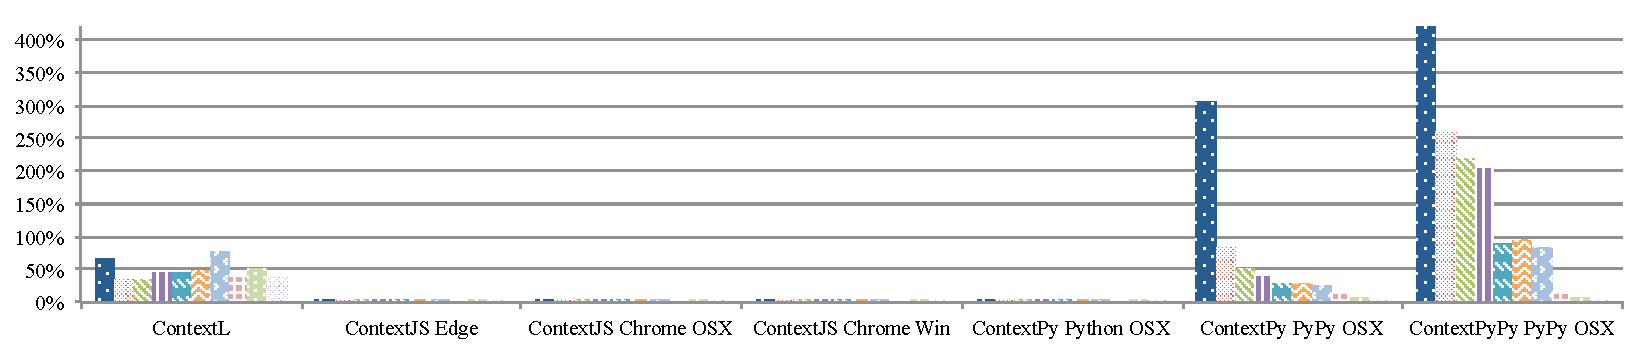
\includegraphics[width=\linewidth]{bench/malte-a/malte-a-1}
  \caption{Bench a overview}
  \label{fig:malte-a-overview}
\end{figure}

%%% Local Variables:
%%% mode: latex
%%% TeX-master: "cop2016-sidewayscomp"
%%% End:


\begingroup
\newcolumntype{P}{S[table-format=3.2]<{{\,\si{\percent}}}}
\begin{table*}
\centering
\caption{Bench A raw ratios}
\smaller
\begin{tabular}{rPPPPPPP}
\toprule
 & \multicolumn{1}{c}{ContextL} & \multicolumn{1}{c}{ContextJS} & \multicolumn{1}{c}{ContextJS} & \multicolumn{1}{c}{ContextJS} & \multicolumn{1}{c}{ContextPy} & \multicolumn{1}{c}{ContextPy} & \multicolumn{1}{c}{ContextPyPy}\\
 & \multicolumn{1}{c}{~} & \multicolumn{1}{c}{Edge} & \multicolumn{1}{c}{Chrome OSX} & \multicolumn{1}{c}{Chrome Win} & \multicolumn{1}{c}{Python OSX} & \multicolumn{1}{c}{PyPy OSX} & \multicolumn{1}{c}{PyPy OSX}\\
\midrule
no activate layer & 67.17 & 0.04 & 0.13 & 0.05 & 3.91 & 300.89 & 444.85\\
1 active layer & 35.90 & 0.09 & 0.09 & 0.03 & 3.93 & 80.40 & 256.90\\
2 active layer & 36.66 & 0.08 & 0.07 & 0.03 & 3.70 & 49.97 & 199.02\\
3 active layer & 43.75 & 0.10 & 0.06 & 0.02 & 3.62 & 40.77 & 206.80\\
4 active layer & 44.90 & 0.08 & 0.05 & 0.04 & 3.50 & 27.18 & 86.63\\
5 active layer & 47.81 & 0.12 & 0.05 & 0.05 & 3.58 & 27.41 & 95.49\\
6 active layer & 77.95 & 0.22 & 0.05 & 0.05 & 3.52 & 26.47 & 86.15\\
7 active layer & 42.77 & 0.18 & 0.06 & 0.05 & 3.50 & 11.42 & 16.04\\
8 active layer & 49.87 & 0.18 & 0.06 & 0.05 & 3.36 & 5.33 & 5.54\\
9 active layer & 37.90 & 0.18 & 0.06 & 0.06 & 3.41 & 4.67 & 4.72\\
\bottomrule
\end{tabular}
\end{table*}


\begin{table*}
\centering
\caption{Bench B raw ratios}
\smaller
\begin{tabular}{rPPPPPPP}
\toprule
 & \multicolumn{1}{c}{ContextL} & \multicolumn{1}{c}{ContextJS} & \multicolumn{1}{c}{ContextJS} & \multicolumn{1}{c}{ContextJS} & \multicolumn{1}{c}{ContextPy} & \multicolumn{1}{c}{ContextPy} & \multicolumn{1}{c}{ContextPyPy}\\
 & \multicolumn{1}{c}{~} & \multicolumn{1}{c}{Edge} & \multicolumn{1}{c}{Chrome OSX} & \multicolumn{1}{c}{Chrome Win} & \multicolumn{1}{c}{Python OSX} & \multicolumn{1}{c}{PyPy OSX} & \multicolumn{1}{c}{PyPy OSX}\\
\midrule
no activate layer & 100.00 & 100.00 & 100.00 & 100.00 & 100.00 & 100.00 & 100.00\\
1 active layer & 74.97 & 91.56 & 50.00 & 71.13 & 86.81 & 105.43 & 85.44\\
2 active layer & 66.25 & 67.17 & 50.00 & 52.01 & 79.57 & 68.73 & 29.64\\
3 active layer & 57.18 & 63.70 & 25.00 & 38.59 & 72.92 & 50.14 & 19.22\\
4 active layer & 22.56 & 53.07 & 25.00 & 29.40 & 66.34 & 38.59 & 14.50\\
5 active layer & 24.72 & 45.31 & 12.50 & 22.74 & 61.86 & 30.54 & 11.30\\
\bottomrule
\end{tabular}
\end{table*}
\endgroup
%%% Local Variables:
%%% mode: latex
%%% TeX-master: "cop2016-sidewayscomp"
%%% End:
